\chapter{Classification of ILP systems}\label{chap:classification_of_ilp_systems}

In the chapter \nameref{chap:issues_in_ilp} we analysed the central issues in ILP by providing a brief explanation of an importance of an issue and a list of the properties defining an issue. In this chapter we classify ILP systems and theoretical frameworks based on the use of the defining properties to approach solving a particar issue.

We will define an ILP task $I \mapsto O$ by its space of possible inputs $I$ and the decription of the desired output $O$. Thus an ILP task is a \emph{function problem} as opposed to a decision problem. We think of an ILP system solving such an ILP task as an \emph{algorithm} computing the function $I \mapsto O$.

\section{ILP task definition}\label{sec:ilp_task_definition}
ILP task definition issue arises from ILP systems using the same \emph{incomplete ILP task definition} although each solves a different machine learning problem.

The objectives of this section are to present the main machine learning problems sought to be solved by ILP systems: generalization and explanatory induction; and then extract their properties upon which a comparison of ILP systems can be based.

We consider defining properties of a machine learning problem: positive examples, negative examples, semantics; that is whose presence or absence in a learning problem is spefified by a corresponding ILP task definition.

\subsection{Generalization}\label{generalization}

\begin{defn}
A theory $T_2$ is \emph{more general} that a theory $T$ wrt the consequence operator $Cn$ iff $Cn(T) \subseteq Cn(T_2)$.
\end{defn}
When the consequence operator $Cn$ is clear or general, we say more succintly that $T_2$ is more general than $T$. Every theory $T$ is more general than itself since $Cn(T) \subseteq Cn(T)$.

\begin{defn}
A theory $T_2$ is \emph{strictly more general} that a theory $T$ wrt the consequence operator $Cn$ iff $Cn(T) \subset Cn(T_2)$.
\end{defn}

\begin{defn}
A learning problem of \emph{generalization} is given a logical theory $T$, find a consistent logical theory $T_2$ more general than the theory $T$ wrt to some consequence operator $Cn$, i.e.
$Cn(T) \subseteq Cn(T_2)$, $false \not\in Cn(T_2)$.
\end{defn}

The objective of generalization is to produce from a theory $T$ a new theory $T_2$ with a greater predictive power to enable logical reasoning about the possible realities with the additional knowledge.

\begin{defn}
Let $T$ be a logical theory. $\phi$ is \emph{predictable} from $T$ iff there is a consistent theory $T_2$ more general than $T$ with $\phi \in Cn(T_2)$. We say that $T_2$ \emph{predicts} $\phi$ from $T$.
\end{defn}

\begin{defn}
A theory $T_2$ is of a \emph{greater predictive power} than $T_1$ iff
for some $T$ it holds that $\forall \phi \in L.$ if $T_2$ predicts $\phi$ from $T$, then $T_1$ predicts $\phi$ from $T_2$ for the language $L$ of the theories $T, T_1, T_2$.
\end{defn}

\begin{exmp}
Let $T$ be a theory $\{mortal(aristotle) \leftObjectImplies man(aristotle), man(adam)\}$. Then the theory $T_2=T \cup \{mortal{adam} \leftObjectImplies man(adam)\}$ is consistent and more general than $T$ assuming a classical consequence operator. $mortal(adam)$ cannot be deduced from the theory $T$ although it can be deduced from its generalized theory $T_2$. Hence $mortal(adam)$ is predictable from $T$.
\end{exmp}

\subsection{Explanatory induction\cite{yamamoto2012inverse}}
\begin{defn}\cite{flach1996rationality} A learning problem of \emph{explanatory induction} is given logical theories background knowledge $B$, examples $E$ to find a hypothesis $H$ satisfying $E \subseteq Cn(B \cup H)$ and $false \not\in Cn(B \cup H)$ for some consequence operator $Cn$.
\end{defn}

This learning problem is alternatively called \emph{learning from entailment}\cite{muggleton1995inverse}\cite{de1997logical}. The examples $E$ can be conceptually divided into positive examples and negative examples $E=E^{+} \cup \neg E^{-}$ where $E, E^{+}, \neg E^{-}$ are conjunctions of logical statements, hence $E^{-}$ being a disjunction of logical statements.

\begin{exmp}\cite{explanatory_induction_example}
Let $E=\{man(adam), \neg man(alice), \neg man(susam)\}$. Then $E^{+}=\{man(adam)\}$,
$\neg E^{-} = \{\neg man(alice), \neg man(susam)\}=\neg man(alice) \land \neg man(susan)$, hence
$E^{-} = man(alice) \lor man(susan)$.
\end{exmp}

Therefore one can define explanatory induction with the negative examples.
\begin{defn}\label{explanatory_induction_with_negative_examples_definition}
A learning problem of \emph{explanatory induction with negative examples} is given logical theories background knowledge $B$, positive examples $E^{+}$, negative examples $E^{-}$ to find a hypothesis $H$ satisfying
$E^{+} \subseteq Cn(B \cup H)$ and $E^{-} \not\in Cn(B \cup H)$.
\end{defn}
The consistency condition has become redundant since $false \in Cn(B \cup H$ implies $E^{-} \in Cn(B \cup H)$.

Explanatory induction is a case of generalization where the theory $T_2=B \cup H$ generalizes the theory $T = B \cup E$.

\subsection{Examples}
Positive examples $E^{+}$ and negative examples $E^{-}$ in explanatory induction put conditions on a possible explanation $H$: $E^{+} \in Cn(B \cup E^{+})$, $E^{-} \not \in Cn(B \cup H)$. As the objective of explanatory induction is to find a good hypothesis explaining the observations from the data, it is important to analyse how the selection of the positive and negative examples affects the learning of a hypothesis.

\subsection{Expressivity}
Additional restrictions on the properties (e.g. \ref{background_representation_of_logic_theories}) of the logical theories on the input and output can make the definition of an ILP task more complete. For example, we may require a logic theory to be a Horn theory, consist at most of one clause or have only terms without function symbols.

\subsection{Semantics}
If two ILP tasks use a different consequence operator, then each specifies a different learning problem and a solution to one of them does not necessarily constitute a solution to the other problem.

\begin{exmp}
Let $Cl$ be a classical consequence operator and $Cp$ be a consequence operator induced by Prolog interpreter. Let $T=\emptyset$, $T_2=\{p\}$.
Then $T_2$ is consistent and more general wrt $Cl$ than $T$. However $T_2$ is not more general wrt $Cp$ than $T$ since $Cp(T) \not\subseteq Cp(T_2)$ as $\neg p \in Cp(T)$ but $p \in Cp(T_2)$.
\end{exmp}

\section{Completeness by problem classes}
A (possibly non-deterministic) ILP task $f:\mathcal{I} \to \mathcal{O}$ as a learning problem can be thought of having deterministic learning subproblems $f':\mathcal{I}' \to \mathcal{O}$ where $\mathcal{I}' \subseteq \mathcal{I}$ and $\forall I \in \mathcal{I}'. f'(I) \in f(I)$. The properties of an input $I \in \mathcal{I}$ and an output $O \in \mathcal{O}$ affect the computation of the output $O$ from an input $I$. Pairs of an input and their unique output with the identical properties create a class of inputs $\mathcal{I}'$ and their unique outputs and therefore solving an ILP task for a class of the inputs $\mathcal{I}'$ and their unique outputs corresponds to the ability to solve a learning subsuproblem $f'$ of an ILP task $f$. The objective of this section is extract the main properties of an input $I$ and its output $O$ to provide the ground for the classification of ILP systems based on their ability to solve a learning subproblem on well-defined class of inputs and their unique outpust in the chapter \fullref{chap:classification_of_ilp_systems}.

For an input $I$ to be compatible with ILP tasks for all ILP systems, an input $I$ of an ILP task of explanatory induction with negative examples \fullref{explanatory_induction_with_negative_examples_definition} is used.

\subsection{Multiplicity of clauses in a hypothesis}
A hypothesis as a clausal theory, can consist of one clause or multiple clauses. Therefore we divide a learning problem $f:\mathcal{I} \to \mathcal{O}$ based on the number of clauses in a possible output for every input $I \in \mathcal{I}$.

\begin{defn}
A learning problem $f:\mathcal{I} \to \mathcal{O}$ is a 
\emph{single clausal} problem iff $\forall I \in \mathcal{I}. \exists O \in f(I). \# O = 1$. That is every input to a problem has a possible output consisting of one clause.
A learning problem that is not single clausal is called a \emph{multi clausal} problem.
\end{defn}

The reader should consult for an example of an input to a single clausal problem \ref{progol_term_structure_learnability}, for an example of an input to a multi clausal problem \ref{progol_multiclausal_learning}.

We classify the ILP systems based on their ability to learn some (not necessarily complete) subclass of multiclausal problems.

\begin{center}
\captionof{table}{Classification by learning multiclausal hypotheses} \label{tab:title} 
\begin{tabular}{| l | l | l | l | l | l | l |}
    \hline
    ILP system & Progol & Aleph & Toplog & Xhail & Imparo & Tal \\ \hline
    Multiclausal& no & yes & no & 
    yes & yes & yes \\ 
     hypotheses & \cite{muggleton2012mc}&\ref{aleph_multiclausal_learning}&
     \cite{muggleton2012mc}&\cite{muggleton2012mc}&\cite{muggleton2012mc}&
     \cite{muggleton2012mc}\\ 
    \hline
\end{tabular}
\end{center}

\subsection{Expressivity of examples}
We classify ILP systems based on whether they can learn explanations for the clausal examples or their observations are limited to atoms.

\begin{center}
\captionof{table}{Classification by learning clausal examples} \label{tab:title} 
\begin{tabular}{| l | l | l | l | l | l | l |}
    \hline
    ILP system & Progol & Aleph & Toplog & Xhail & Imparo & Tal \\ \hline
    Clausal& yes & no & no & 
    no & no & no \\ 
     examples & \ref{progol_clausal_examples} &\cite{aleph2007}&
     \ref{toplog_clausal_examples}&
     \ref{imparo_clausal_examples}&\ref{tal_clausal_examples}\\
    \hline
\end{tabular}
\end{center}

Xhail cannot learn clausal examples as all examples have to be in a body of a goal to be proved as seen in the appendix, therefore examples need to be literals.

\subsection{Generalization downwards}
\begin{center}
\captionof{table}{Classification by generalization downwards} \label{tab:title} 
\begin{tabular}{| l | l | l | l | l | l | l |}
    \hline
    ILP system & Progol & Aleph & Toplog & Xhail & Imparo & Tal \\ \hline
    & no & yes & no &  & no & no \\ \hline
    & & & & & & \\ \hline
\end{tabular}
\end{center}

\subsection{Double Kleene star}
\begin{center}
\captionof{table}{Classification by double Kleene star operator} \label{tab:title} 
\begin{tabular}{| l | l | l | l | l | l | l |}
    \hline
    ILP system & Progol & Aleph & Toplog & Xhail & Imparo & Tal \\ \hline
    & no & no & no & & yes & yes \\ \hline
    & & & & & & \\ \hline
\end{tabular}
\end{center}

\section{Bias}
ILP systems use bias to refine their search space $\mathcal{H}$, to induce a preference relation on the space of hypotheses and to control their search. The objective of this section is to classify the ILP systems based on the biases they use and the capabilities of their biases of a certain type.

\subsection{Language bias}\label{subsec:classification_language_bias}
The objective of this subsection is to classify ILP systems based on their peculiarities related to the language bias: mode declarations, determinations and metaconstraints.

\subsubsection{Mode declarations}
The use of the mode declarations in an ILP system and their defining role is summarised.

We examine the compatibility of mode declarations with the mode declarations of Progol since mode declarations were first defined for Progol in seminal work by Muggleton\cite{muggleton1995inverse}.
We say that a system of mode declarations is Progol compatible iff any hypothesis bias definable with Progol mode declarations can be defined within that system.

\captionof{table}{Classification by mode declaration bias} \label{tab:classification_by_mode_declaration_bias} 
 \begin{tabular}{| l | l | l | l | l | l | l |}
    \hline
    Mode declarations/ILP system & Progol & Aleph & Toplog & Xhail & Imparo & Tal \\ \hline
    Progol compatible & yes & yes & no &  yes & no & no \\ \hline
    Recall modeb support & yes & yes & yes & yes & no & yes \\ \hline
    Recall modeh support & yes & yes & no & yes & no & no \\ \hline
    Recall lower bound support & no & no & no & yes & no & no \\ \hline
  \end{tabular}

The author further supports the statements in a summary by examining a system of mode declarations for each ILP system.

\paragraph{Progol}
Progol supports the mode declarations as defined in \fullref{background_mode_declarations}.

\begin{exmp}\cite{muggleton1999progolWebsite}
\begin{lstlisting}
:- modeh(1,class(+animal,#class))?
:- modeb(1,has_gills(+animal))?
:- modeb(*,habitat(+animal,#habitat))?
:- modeh(1,append([+constant|+clist],+clist,[-constant|-clist]))?
:- modeh(1,append(+clist,+clist,-clist))?
\end{lstlisting}
\end{exmp}

\paragraph{Aleph}
Aleph's mode declarations are compatible\cite{aleph2007} with the mode declarations specified by Progol.
\begin{exmp}
\begin{lstlisting}

:-modeh(1, woman(+person)).
:-modeb(1, female(+person)).
:-modeb(*, english_couple(+person, -person)).
:-modeb(2, english(+person)).
\end{lstlisting}
\end{exmp}

\paragraph{Toplog}
Toplog's modeb declarations are compatible with Progol up to specification of the atom. Specification of the recall is optional, however, for modeh declarations recall cannot be specified\cite{santos2008toplogWebsite}.
\begin{exmp}\cite{santos2008toplogWebsite}
\begin{lstlisting}
:-modeh(append(+list,+list,-list)).
:-modeb(append(+list,+list,-list)).
:-modeb(5,append(+list,+list,-list)).
:-modeh(class(+animal,#class)).
:-modeh(*,uncle(+person, -person)).%invalid
\end{lstlisting}
\end{exmp}

\paragraph{Xhail}\label{xhail_mode_declarations}
Xhail has extended mode declarations to include metaconstraint statements in order to refine its search space.

Xhail executable's help\cite{ray2007xhail} reads:
\begin{quote}
\emph{Zero or more head declarations} are of the form
\tc{modeh(1,3,min,p("\#q","+r","-s"))} meaning between 1 and 3 ground atoms
 of the form $p(a,b,c)$ should be assumed such that $q(a), r(b), s(c)$ hold 
 and where $a, b, c$ are constant, input, output terms, respectively;
 the third flag is either min="attempt to minimize" or all="do not minimize".
 
\emph{Zero or more body declarations} are of the form \tc{modeb(1,3,pos,p("\#q","+r","-s")).} meaning this scheme can be used between 
 depths 1 and 3.  The third flag is either pos="pos. literal" or neg="neg. literal" 
\end{quote}

\begin{exmp}\ref{xhail_fine_search_space_control}
\begin{lstlisting}
modeh(0,1,all,woman("+person")).
modeb(0,1,pos,female("+person")).
\end{lstlisting}
\end{exmp}

Whereas Progol specifies the recall by its upper bound, Xhail enables its specification for both its \emph{lower bound} and upper bound. Metaconstraint statements
\tc{min}, \tc{all}, \tc{pos}, \tc{neg} constraint the hypothesis bias further.

\paragraph{Imparo}\cite{kimber2013imparo}
Imparo does not support recall specification in its mode declarations. The specification of the atom is supported.
\begin{exmp}
\begin{lstlisting}
head_modes([
    woman(+number)
]).
body_modes([
    female(+number)
]).
\end{lstlisting}
\end{exmp}

\paragraph{Tal}
Tal does not support recall specification for modeh declarations, however the recall can be specified for the modeb declarations\cite{corapi2011tal}.
\begin{exmp}
\begin{lstlisting}
modeh(happens("#event","#time","#scenario")).
modeh(woman(+person), [name(wh)]).
modeb(female(+person), [name(fb)]).
modeb(2,female(+person), [name(fb)]).
\end{lstlisting}
\end{exmp}

\subsubsection{Determinations}
By reading the manuals of the corresponding ILP systems, one may find that
Toplog, Xhail, Imparo, Tal do not support the determinations.
Progol supports the use of the determinations, cf. \ref{progol_multiclausal_learning}, but it does not require it, cf. \ref{progol_specialization_in_arguments}.
Aleph requires the determinations to be specified\fullref{subsec:aleph_determination_declaration_requirement}.

\subsubsection{Metaconstraints}
Metaconstraints supplement mode declarations and determinations in specifying the language bias. Several metaconstraints are selected and their support is evaluated accross the ILP systems classified:

\begin{itemize}
\item the maximum number of literals in a clause of a hypothesis,
\item the maximum number of clauses in a hypothesis - some incomplete ILP systems do not support multiclausal hypotheses, therefore they do not need and cannot support this metaconstraint,
\item the maximum variable depth\ref{definition_variable_depth} of a hypothesis,
\item the (minimum and maximum) number of singletons in a hypothesis:
a singleton is a variable that appears only once in a hypothesis\cite{santos2008toplogWebsite}
\end{itemize}

\begin{defn}\label{definition_variable_depth}\cite{nienhuys1997foundations}
The \emph{variable depth of a variable} $x$ in an ordered definite program clause
$A \leftObjectImplies  B_1, . . . , B_n$ is defined as follows. If $x$ occurs in $A$, then its variable depth is $0$. Suppose $x$ first occurs in $B_i$.
If none of the other variables
in $B_i$ already occurred in $A \leftObjectImplies B_1,... ,B_{i-1}$,
then $x$ has variable depth $\infty$.
Otherwise, the variable depth of $x$ is $1$ plus the variable depth of the variable in $B_i$ with greatest variable depth occurring in
$A \leftObjectImplies B_1,... ,B_{i-1}$.
The \emph{variable-depth of a clause} in an ordered definite program
is the largest variable depth of its variables. Note that such a
clause is constrained iff it has variable depth $0$.
\end{defn}

\begin{exmp}
Let $H=path(X,Y) \leftObjectImplies path(X,X_1), arc(X_1,X_2), path(X_2,Y)$.
Then the variable depths of the variables $X,Y,X_1,X_2$ in $H$ are
$0,0,1,2$ respectively.
\end{exmp}

\paragraph{Progol}
Progol can learn only single-clausal hypotheses\cite{muggleton2012mc}, therefore it does not support a metaconstraint specifying the number of clauses in a hypothesis.
Prolog manual does not provide information about its metalevel constraints. The metalevel constraints used in the provided files\cite{muggleton1999progolWebsite} were of the following format:
\begin{lstlisting}
./pole.pl::- op(10, xfx, ...)?
./pole.pl::- op(30,xfy,:)?
./numbers.pl::- set(h,100)?
./numbers.pl::- set(r,1000)?
./numbers.pl::- set(inflate,99)?
./numbers.pl::- set(nodes,100)?
./numbers.pl::- set(i,5), set(c,5)?
\end{lstlisting}
Their change did not affect the properties examined, hence the author assumes Progol does not support any of the metaconstraints.

\paragraph{Aleph}
Aleph supports the first 3 chosen metaconstraints as can be consulted in the section 18 of the Aleph manual\cite{aleph2007}.
\begin{quote}
\begin{itemize}
\item (Maximum number of literals in a clause) \tc{set(clauselength,+V)}:
$V$ is a positive integer (default $4$). Sets upper bound on number of literals in an acceptable clause.
\item (Maximum number of clauses in a hypothesis) \tc{set(clauses,+V)}:
$V$ is a positive integer. Sets upper bound on the number of clauses in a theory  when performing theory-level search.
\item (Variable depth) \tc{set(i,+V)}: $V$ is a positive integer (default $2$). Set upper bound on layers of new variables.
\end{itemize}
\end{quote}

The manual does not provide the information on specifying the number of singletons in a clause, hence it is assumed that this feature is not supported.

\paragraph{Toplog}
Toplog can learn only single-clausal hypotheses\cite{muggleton2012mc}, therefore it does not support a metaconstraint specifying the number of clauses in a hypothesis. It supports the specification of the maximum number $N$ of literals in a hypothesis with a metalevel statement\\
\tc{:-set(maximum\_literals\_in\_hypothesis,N)} found for example in carcinogenesis.pl file\cite{santos2008toplogWebsite}. The manual does not provide any information on the variable depth, therefore it is assumed that this feature is not supported in Toplog.
By the manual Toplog supports the specification of a maximum and minimum number of singletons in a hypothesis as can be also found in carcinogenesis.pl file:
\begin{lstlisting}
:-set(maximum_singletons_in_hypothesis,3)%carcinogenesis.pl
:-set(maximum_literals_in_hypothesis,4).%carcinogenesis.pl
\end{lstlisting}

\paragraph{Xhail}
In \ref{xhail_mode_declarations} we found out that Xhail has the most advanced system of mode declarations. On the other hand it does not support any of the chosen metaconstraints\cite{ray2007xhail}. The author consulted the Xhail's help and example files provided with Xhail as there was no access to the source code.

\paragraph{Imparo}
In a grammar learning file available with Imparo\cite{kimber2013imparo} one can find the setting:
\begin{lstlisting}
:-set_max_clause_length(6).
:-set_max_clauses(1).
:-set_max_var_depth(4).
\end{lstlisting}
Therefore Imparo supports the specification of the clausal length, the maximum number of clauses in a hypothesis and the maximum variable depth of a clause in a hypothesis. Imparo's manual and source code do not provide any information on bounding the number of singleton variables in a clause, hence it is assumed this feature is not supported.

\paragraph{Tal}
Tal enables the specification of the clausal length by specifying the number of the literals in the body of a clause \tc{option(max\_body\_literals, N)}\cite{corapi2010inductive}. Tal specifies the number of clauses in a hypothesis with \tc{option(max\_num\_rules, N)}\cite{corapi2010inductive}, where a rule is understood as a clause. Tal's manual and source files do not mention variable depth and bounding the number of singleton variables in a clause, hence it is assumed that these features are not supported.

\paragraph{Summary}
The support for the metaconstraints of interest is summarised.

\captionof{table}{Classification by metaconstraints} \label{tab:classification_by_metaconstraints} 
 \begin{tabular}{| l | l | l | l | l | l | l |}
    \hline
    Metaconstraint/ILP system & Progol & Aleph & Toplog & Xhail & Imparo & Tal \\ \hline
    Max. no. of literals in a clause & no & yes & yes & no & yes & yes\\ \hline
    Max. no. of clauses in $H$ & no & yes & no & no & yes & yes\\ \hline
    Max. variable depth in $H$ & no & yes & no & no & yes & no\\ \hline
    Number of singletons in $H$ & no & no & yes & no & no & no\\ \hline
  \end{tabular}
  
If one considered the chosen metaconstraints as representative, then it could be deduced that Progol and Xhail have the most trivial system of specifying the language bias with metaconstraints whereas Aleph and Imparo have the most poweful system.

\section{Hypothesis search}
Hypothesis search concerns with the algorithms used for searching a hypothesis, their heuristics, search biases and other search control mechanisms.
First we list a hypothesis search algorithm for each ILP system and then 
we compare how ILP systems search the hypothesis space based on the properties:
\begin{itemize}
\item search direction.
\end{itemize}

\subsection{Algorithms}

\subsubsection{Progol\cite{muggleton1995inverse}\cite{kimber2012learning}}
Progol's algorithm consists of steps:
\begin{itemize}
\item initialize $H$ to be an empty theory,
\item step 2: if $E=\emptyset$ then return $H$,
\item select an example $e \in E$,
\item construct a most specific clause within the mode language which entails $e$,
\item specialise the $\bot$ clause searching down the lattice using the A*-heuristics until a clause $h$ explaining $e$ is found, then add $h$ to $H$,
\item use the cover loop algorithm to remove all the examples from $E$ that are already explained by $H$ so far and go to step 2.
\end{itemize}

\subsubsection{Aleph}
In the Aleph manual\cite{aleph2007} a reader would find the description of the basic algorithm:
\begin{enumerate}
\item \emph{Select example.} Select an example to be generalised. If none exist, stop, otherwise proceed to the next step.
\item \emph{Build most-specific-clause.} Construct the most specific clause that entails the example selected, and is within language restrictions provided. This is usually a definite clause with many literals, and is called the "bottom clause." This step is sometimes called the "saturation" step. Details of constructing the bottom clause can be found in Stephen Muggleton's 1995 paper: Inverse Entailment and Progol\cite{muggleton1995inverse}.
\item \emph{Search.} Find a clause more general than the bottom clause. This is done by searching for some subset of the literals in the bottom clause that has the "best" score. Two points should be noted. First, confining the search to subsets of the bottom clause does not produce all the clauses more general than it, but is good enough for this thumbnail sketch. Second, the exact nature of the score of a clause is not really important here. This step is sometimes called the "reduction" step.
\item \emph{Remove redundant.} The clause with the best score is added to the current theory, and all examples made redundant are removed. This step is sometimes called the "cover removal" step. Note here that the best clause may make clauses other than the examples redundant. Again, this is ignored here. Return to Step 1.
\end{enumerate}

\subsubsection{Toplog\cite{muggleton2008toplog}\cite{corapi2011nonmonotonic}}
The Toplog algorithm used to find a hypothesis $H$ uses an extended inverse entailment following the steps:

\begin{itemize}
\item construct the top theory $\top$,
\item for every example $e \in E$:
\item derive a clause $h_e$ such that $\top \models h_e$, $B \cup \{h_e\} \models e$, add $h_e$ to $H_c$,
\item end loop,
\item select $H \in H_c$ such that $s(H)$ is maximized for a score function $s:\mathcal{H} \to \mathbb{R}$.
\end{itemize}
The score function can be based on compression, coverage, accuracy, etc.

\subsubsection{Xhail}


\subsubsection{Imparo}
Imparo is an ILP system based on a general IoF theoretical framework with the following algorithm:
\begin{itemize}
\item 1: select an example $E$ from the set of positive examples $E_{pos}$,
\item compute the most specific connected theory for an example $E$ and the background knowledge $B$,
\item search the lattice of sets of clauses subsuming the connected theory and choose the hypothesis $H$ with the highest score according to the score function such that $H \models E$,
\item add $H$ to $B$,
\item remove all $E' \in E_{pos}$ implied by new $B$, $B \models E'$.
\item if $E_{pos} = \emptyset$ finish, otherwise go to 1.
\end{itemize}

\paragraph{Induction on Failure framework\cite{kimber2012learning}}
Induction on Failure framework (IoF) is a method for deriving a hypothesis $H$ where a single clause $h \in H$ does not necessarily need to explain an example $e \in E$, but an example can be explained by multiple clauses. Such a search space is called a connected theory.
\begin{defn}
A connected theory $T$ for a ground Horn clause $e$ and a Horn theory $B$ is a set of clauses that can be partitioned into sets $T_1, ..., T_n$ so that
(i) $B \union T_1^+ \models e_{head}$,
(ii) $\forall i \in \{1, ..., n-1\}. B \union e_{body} \union T_{i+1}^+ \models T_i^-$,
(iii) $B \union e_{body} \models T_n^-$,
(iv) $B \union T \not\models \square$.
\end{defn}

\subsubsection{Imparo\cite{kimber2012learning}}

\subsubsection{Tal}

\subsection{Search direction\cite{nienhuys1997foundations}}
When searching for a correct hypothesis \ref{correct_hypothesis}, one may either start with an overly general hypothesis $H$ wrt $B, E^+$, $E^-$ and then try to weaken it to make it consistent with the negative examples $E^-$ while preserving its completeness wrt positive examples $E^+$. This is called a \emph{top-down} search.
On the other hand, in a \emph{bottom-up} search one starts with an overly specific hypothesis $H$ wrt $B$, $E^+$, $E^-$ and then tries to strengthen it to make it complete wrt positive examples $E^+$ while preserving the consistency wrt to the negative examples $E^-$.
The combination of both search strategies results in a \emph{mixed} search.

\begin{remark}
A reader should be careful. In the contemporary literature there are other notions and respective classes of bottom-up and top-down systems (c.f.\cite{corapi2010inductive} for Toplog). We follow the classification by Nienhuys-Cheng and Wolf\cite{nienhuys1997foundations}.
\end{remark}

We classify ILP systems based on their direction of search.

\begin{center}
\captionof{table}{Classification by hypothesis search direction}\label{tab:title} 
\begin{tabular}{| l | l | l | l | l | l | l |}
    \hline
    ILP system & Progol & Aleph & Toplog & Xhail & Imparo & Tal \\ \hline
   	Search direction & top-down & bottom-up& mixed & bottom-up & mixed & top-down\\ \hline
\end{tabular}
\end{center}

\begin{center}
\captionof{figure}{Top-down and bottom-up direction of hypothesis search}
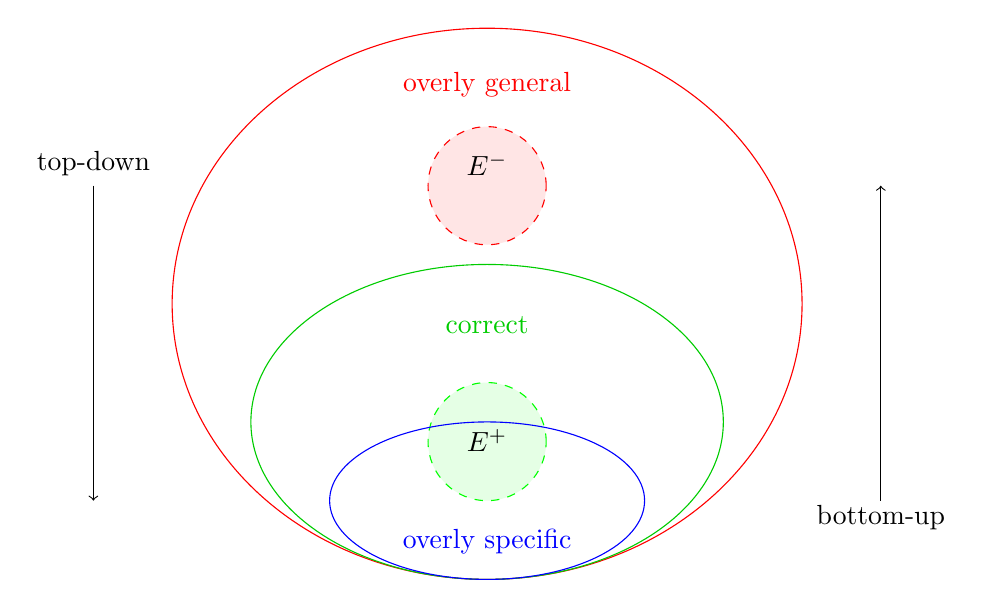
\begin{tikzpicture}
\draw[color=green, style=dashed, fill=green!10] (7, 1.75) circle (0.75);
\draw[color=red, style=dashed, fill=red!10] (7, 5) circle (0.75);
\draw[color=red] (7,3.5) ellipse (4 and 3.5);
\draw[color=green!80!black] (7,2) ellipse (3 and 2);
\draw[color=blue] (7,1) ellipse (2 and 1);
\fill (7,1.5) node[above] {$E^+$};
\fill (7,5) node[above] {$E^-$};
\fill[color=red] (7,6) node[above] {overly general};
\fill[color=green!80!black] (7,3) node[above] {correct};
\fill[color=blue] (7,0.2) node[above] {overly specific};
\draw [->] (12,1) -- (12,5);
\draw [->] (2,5) -- (2,1);
\fill (2,5) node[above] {top-down};
\fill (12,0.5) node[above] {bottom-up};
\end{tikzpicture}
\end{center}

\paragraph{Progol}
Progol searches top-down for hypotheses that subsume some bottom clause.\cite{nienhuys1997foundations}.
\paragraph{Aleph\cite{aleph2007}}
Although Aleph being based on Progol, it searches a hypothesis bottom-up. It first selects an example to be generalized, finds a bottom clause that entails it, then it generalizes the bottom clause further until a correct hypothesis is found.
\paragraph{Toplog\cite{muggleton2008toplog}}
Corapi\cite{corapi2011nonmonotonic} surveys that Toplog derives all the hypotheses $H_e$ that are generalizations of some positive example $e \in E^+$ constructing a set $H_c=\{h_e:e \in E^+\}$.
Afterwards a subset $H \in H_c$ maximizing a score function is chosen. Strictly in this sense Toplog does not perform a search. The first step of generalization is analogous to a bottom-up search. Based on the score function the second step of selection may eliminate overly general hypotheses and is therefore analogous to a top-down search. We conclude that Toplog uses a mixed hypothesis search strategy.
\paragraph{Xhail\cite{ray2003hybrid}}
Xhail (based on Hail) constructs a kernel set from the background knowledge $B$ and an example $e$ which is subsequently generalized until a correct hypothesis is found. Therefore Xhail searches a hypothesis $H$ bottom-up.

\paragraph{Imparo}
Imparo is based on the induction on failure (IoF) framework:
\begin{quote}\cite{kimber2012learning}
The procedure[IoF] interleaves top-down subsumption-based search with bottom-up generalisation of the ground connected theory T .
\end{quote}
Therefore Imparo uses a mixed strategy to search for a hypothesis.
\paragraph{Tal}
We conclude that Tal searches a hypothesis top-down from the quote bellow:
\begin{quote}\cite{corapi2010inductive}
Tal explores candidate solutions in a top-down manner,
backtracking whenever the current solution leads to failure in the abductive derivation.
\end{quote}

\section{Robustness}
We classify ILP systems based on whether they check for the consistency of the input theories and whether they always terminated.

\begin{center}
\captionof{table}{Classification by robustness} \label{tab:title} 
\begin{tabular}{| l | l | l | l | l | l | l |}
    \hline
    ILP system & Progol & Aleph & Toplog & Xhail & Imparo & Tal \\ \hline
    Consistency check & yes & no & no & yes & no & no \\
	& \ref{progol_consistency_check}
	& \ref{aleph_consistency_assumption}
	& \ref{toplog_consistency_assumption}
	 & \ref{xhail_implicit_consistency_check}
	 & \ref{imparo_consistency_assumption}
	 & \ref{tal_consistency_assumption} \\ \hline
    Always terminated & yes & yes & yes & yes & no & no \\ 
	&  & & & & \ref{imparo_clausal_examples} & \ref{tal_loop_on_learning_regular_languages} \\ \hline
\end{tabular}
\end{center} 

The property ``Always terminated'' evaluates whether an ILP system terminated on all the experiments in the appendix. However, it may be possible for a system that withstood our experiments that one could find an input on which a system would not terminate. Therefore this test is only indicative.